\rhead{8. Dijagrami sekvence}
\section{Dijagrami sekvence}
\par U nastavku se nalaze dijagrami sekvence korišćeni za analizu interakcija u sistemu. Opisana su 4 dijagrama sekvence:
\begin{itemize}
    \item \textbf{Promocija u volontera}
    \item \textbf{Pregled novih objava}
    \item \textbf{Udomljavanje}
    \item todo
\end{itemize}
\subsection{Promocija u volontera}
\par \textit{Član} može da postane \textit{volonter} tako što pošalje zahtev za volonterstvo. Svaki \textit{volonter} može da glasa samo jednom dokle god traje glasanje. 
Na kraju glasanja, status zahteva se menja u zavisnosti od broja glasova. Da bi zahtev bio prihvaćen,
potrebno je da 50\% glasača budu za promociju. Ukoliko je zahtev prihvaćen članu se menja status. Ovo je prikazano na dijagramu \ref{fig:promotion-seq}.
\begin{figure}[h]
    \centering
    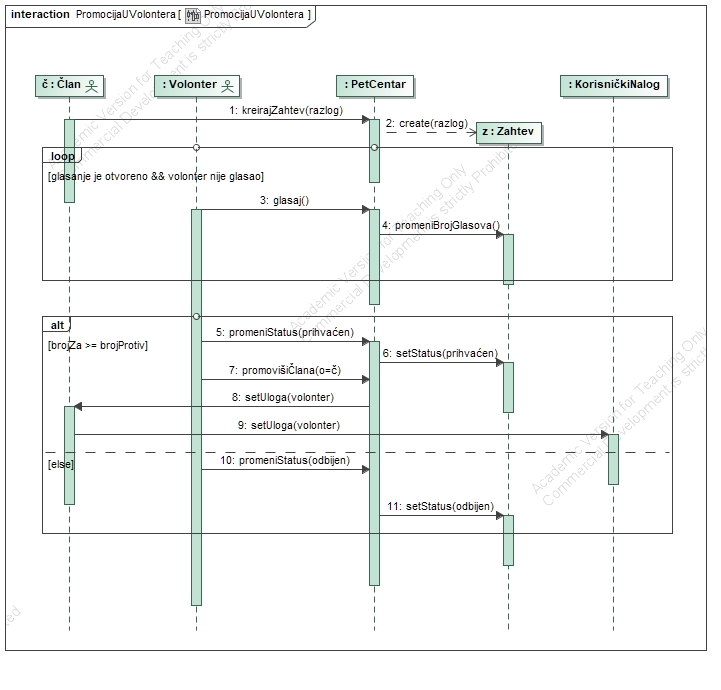
\includegraphics[width=\textwidth, height=0.9\textwidth]{img/promote-member-sequence.jpg}
    \caption{Dijagram sekvence za promociju u volontera}
    \label{fig:promotion-seq}
\end{figure}
\subsection{Pregled novih objava}
\par \textit{Volonter} može da vidi sve objave koje su na čekanju. Nakon prikaza, on može da prihvati ili odbije ponudu. U zavisnosti od odluke, menja se
stanje objave i briše prethodno stanje (\textit{NaČekanju}). Ovo je prikazano na dijagramu \ref{fig:posts-list-seq}.
\begin{figure}[h]
    \centering
    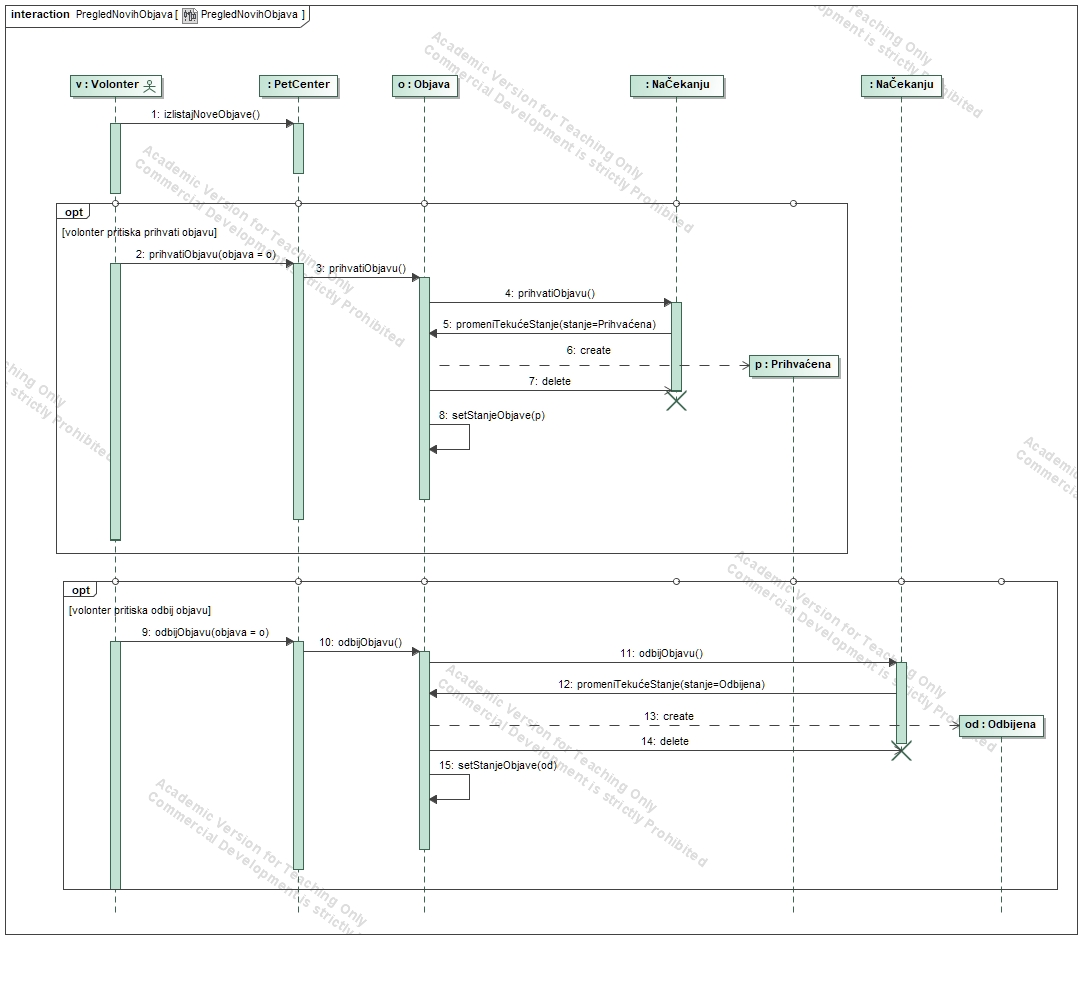
\includegraphics[width=\textwidth, height=\textwidth]{img/new_posts-sequence.jpg}
    \caption{Dijagram sekvence za pregled novih objava}
    \label{fig:posts-list-seq}
\end{figure}
\subsection{Udomljavanje}
\par \textit{Član} može da udomi životinju tako što kreira ponudu [Dijagram \ref{fig:activity-send-offer}]. \textit{Volonter} ima uvid u sve ponude i može da
prihvati i odbije. Ukoliko je ponude prihvaćena, stanje objave se menja u \textit{udomljena}. U suprotnom, stanje objave ostaje isto, ali se menja u 
ponudi na \textit{odbijena}.
\begin{figure}[ht]
    \centering
    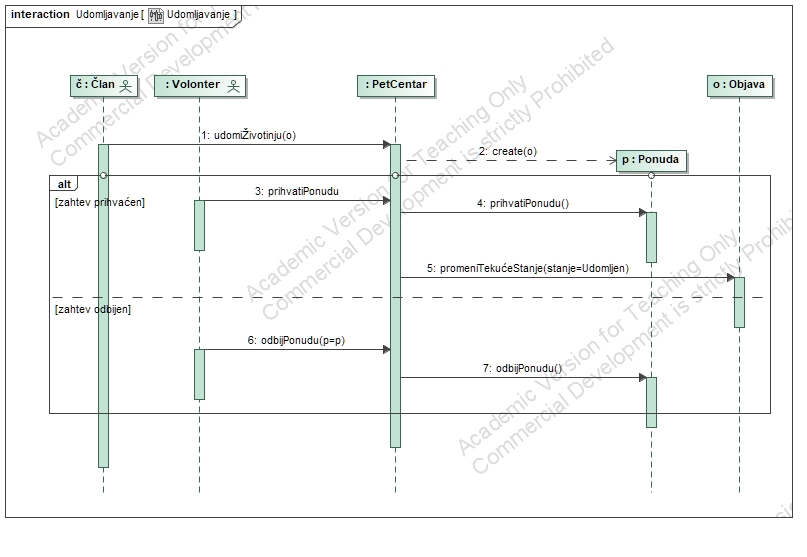
\includegraphics[width=\textwidth, height=\textwidth]{img/adoption.jpg}
    \caption{Dijagram sekvence za udomljavanje}
    \label{fig:adoption-seq}
\end{figure}